\newif\ifglobal

%%%%%%%%%%%%%%%%%%%%%%%
%%% Compile to view %%%
%%%%%%%%%%%%%%%%%%%%%%%

%%%%%%%%%%%%%%%%%%%%%%%%%%%%%%%%%%%%%%%%%%%%%%%%%%%
%%% Readme:                                     %%%
%%% https://www.overleaf.com/read/bwdjvfjksvjy/ %%%
%%%%%%%%%%%%%%%%%%%%%%%%%%%%%%%%%%%%%%%%%%%%%%%%%%%

% >>> M?: marks a module setting number or important notice

% >>> M4: Set {./relative-path} to external files for this module <<<
\def \modulefiles {./09-RESCLK}
% To add an external file, use:
% (Replace '---' with actual filename)
% '\input{\modulefiles/tables/---.tex}' for tables
% '\includegraphics{\modulefiles/figures/---}' for figures
% '\subfile{\modulefiles/---}' for register files


% >>> M1: This module is in global project? <<<
% 'YES' - uncomment; 'NO' - comment out
\globaltrue

\ifglobal
    \documentclass[main\_\_CN.tex]{subfiles}

\else
    % Font "FandolSong-Regular" used by ctex does not have GSUB table.
    % It causes warnings that do not affect compilation and can be ignored.
    \PassOptionsToPackage{quiet}{fontspec}

    \documentclass[openany, 10pt]{book}

    % >>> M2: In ./00-shared/preamble-trm-module, also find
    %         settings for visibility of todo notes, watermark <<<
    \usepackage{preamble-trm-module}


    % Enable Chinese typesetting
    \usepackage{ctex}

    % >>> M3: Temporary labels in Chinese
    %         you can add your own labels there <<<
    \myexternaldocument{./00-shared/temp-labels-cn}

\fi %\ifglobal


\setcounter{secnumdepth}{4}


% >>> M5: If this module needs any updates in
% './00-shared/preamble-trm-module.sty'
% (include additional package, etc.), contact your module PM
% or create the file './00-shared/changelog.tex' make the
% necessary updates yourself and document them in this file <<<


\begin{document}


% Sets language into which pre-defined bits of text are translated
\selectlanguage{chinese}

% Do not delete this block
\ifglobal
% Add the following front matter if
% this module is outside of global project
\else
    \InputIfFileExists{readme}{}{}
    {\let\clearpage\relax \listoftodos}
    {\let\clearpage\relax \listofdonetodos}
    \tableofcontents
    %\listoftables
    %\listoffigures
\fi

%%%%%%%%%%%%%%%%%%%%%%%%%
%%% TRM Module Begins %%%
%%%%%%%%%%%%%%%%%%%%%%%%%

\hypertarget{resclk}{}
\chapter{复位和时钟}
\label{mod:resclk}




\section{复位}
\subsection{概述}
\chipname{} 提供四种级别的复位方式，分别是 CPU 复位、内核复位、系统复位和芯片复位。除芯片复位外，其他复位方式不影响片上内存存储的数据。图 \ref{figure:Reset} 展示了整个芯片系统的结构以及四种复位等级。

\subsection{结构图}
\begin{figure}[H]
    \centering
    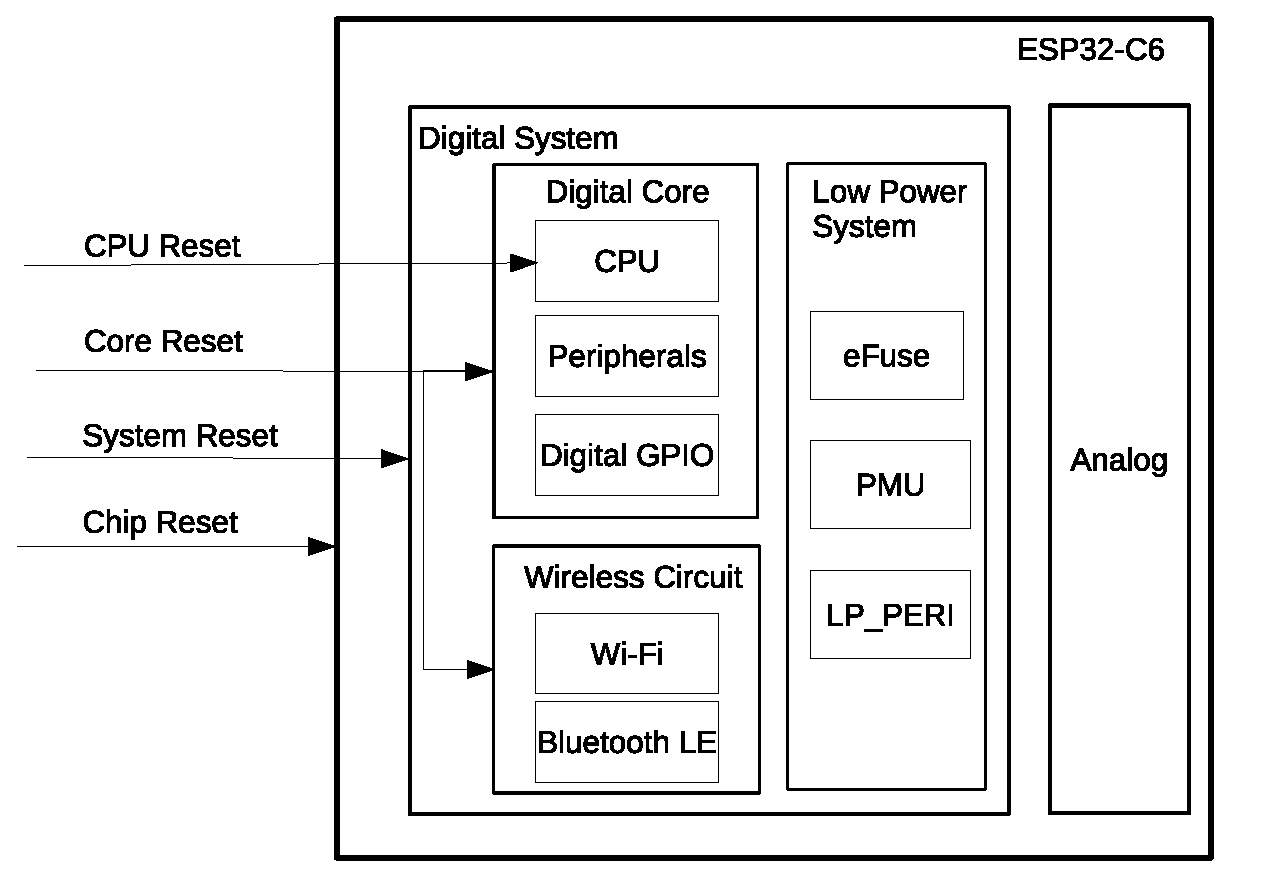
\includegraphics[width=0.8\textwidth]{./09-RESCLK/figures/reset-overview-20220821.eps}
    \caption{四种复位等级}
    \label{figure:Reset}
\end{figure}
芯片的数字系统分为两部分：\hyperref[mod:riscvcpu]{高性能系统 (High Performance System, HP system)} 和 \hyperref[mod:ulp]{低功耗系统 (Low Power System, LP system)}。其中高性能系统包含数字内核 (Digital Core) 和无线电路 (Wireless Circuit)。 详细信息可参考图 \ref{figure:Reset}。


\subsection{特性}
\label{sec:resclk-features}
\begin{itemize}
    \item 支持四种复位等级：
    \begin{itemize}
    \item CPU 复位：复位 CPU 核。复位释放后，程序将从 CPU Reset Vector 开始执行；
    \item 内核复位：复位除低功耗系统以外的其他数字系统，包括 CPU、外设、Wi-Fi、Bluetooth$^®$ LE 及数字 GPIO；
    \item 系统复位：复位包括低功耗系统在内的整个数字系统；
    \item 芯片复位：复位整个芯片。
    \end{itemize}
    \item 支持软件复位和硬件复位：
    \begin{itemize}
        \item 软件复位：CPU 配置相关寄存器可触发软件复位，见章节 \ref{mod:lowpowm} \textit{\nameref{mod:lowpowm}}；
        \item 硬件复位：硬件复位直接由硬件电路触发。
    \end{itemize}
\end{itemize}



\subsection{功能描述}
上述任一复位发生时，CPU 将立刻复位。复位释放后，CPU 可通过读取 \hyperref[fielddesc:RTCCLKRSTRESETCAUSE]{RTC\_CLKRST\_RESET\_CAUSE} 获取复位源。

表 \ref{tab:resclk-reset-src} 列出了从上述寄存器中可能读出的复位源及其触发的复位等级。

\begin{table}[H]
    \centering
    \caption{复位源}
    \label{tab:resclk-reset-src}
    \begin{threeparttable}
    \begin{tabular}{ |l|m{3.5cm}|m{1.8cm}|m{9.2cm}| }
    \hline
\rowcolor{lightgray}
\textbf{编码} & \textbf{复位源} & \textbf{复位等级} &   \textbf{说明} \\\hline
        0x01 & 芯片复位\tnote{1} & 芯片复位 & ---\\
        \hline
        0x0F & 欠压系统复位 & 芯片复位或系统复位 & 欠压检测器触发的复位\tnote{2}\\
        \hline
        0x10 & RWDT 系统复位 & 系统复位 & 详见章节 \ref{mod:wdt} \textit{\nameref{mod:wdt}}
        \\\hline
        0x12 & 超级看门狗复位 & 系统复位 & 详见章节 \ref{mod:wdt} \textit{\nameref{mod:wdt}}
        \\\hline
        0x03 & 软件系统复位 & 内核复位 & 配置 \hyperref[fielddesc:LPAONHPSYSSWRESET]{LP\_AON\_HPSYS\_SW\_RESET} 触发\\
        \hline
        0x05 & Deep-sleep 复位 & 内核复位 & 详见章节 \ref{mod:lowpowm} \textit{\nameref{mod:lowpowm}}
        \\\hline
        0x06 & SDIO 内核复位 & 内核复位 & 保留
        \\\hline
        0x07 & MWDT0 内核复位 & 内核复位 & 详见章节 \ref{mod:wdt} \textit{\nameref{mod:wdt}}
        \\\hline
        0x08 & MWDT1 内核复位 & 内核复位 & 详见章节 \ref{mod:wdt} \textit{\nameref{mod:wdt}}
        \\\hline
        0x09 & RWDT 内核复位 & 内核复位 & 详见章节 \ref{mod:wdt} \textit{\nameref{mod:wdt}}
        \\\hline
        0x14 & eFuse 复位 & 内核复位 & eFuse CRC 校验错误触发复位
        \\\hline
        0x15 & USB (UART) 复位 & 内核复位 & 外部 USB 主机发送特定命令给 USB Serial/JTAG 控制器的 Serial 接口将触发此复位，详见章节 \ref{mod:usbserialjtag} \textit{\nameref{mod:usbserialjtag}} \\\hline
        0x16 & USB (JTAG) 复位 & 内核复位 & 外部 USB 主机发送特定命令给 USB Serial/JTAG 控制器的 JTAG 接口将触发此复位，详见章节 \ref{mod:usbserialjtag} \textit{\nameref{mod:usbserialjtag}} \\\hline
        0x0B & MWDT0 CPU 复位 & CPU 复位 & 详见章节 \ref{mod:wdt} \textit{\nameref{mod:wdt}}
        \\\hline
         0x0C & 软件 CPU 复位 & CPU 复位 & 配置 \hyperref[fielddesc:LPAONCPUCORE0SWRESET]{LP\_AON\_CPU\_CORE0\_SW\_RESET} 触发\\
        \hline
        0x0D & RWDT CPU 复位 & CPU 复位 & 详见章节 \ref{mod:wdt} \textit{\nameref{mod:wdt}}
        \\\hline
        0x11 & MWDT1 CPU 复位 & CPU 复位 & 详见章节 \ref{mod:wdt} \textit{\nameref{mod:wdt}}
        \\\hline
        0x18 & JTAG CPU 复位 & CPU 复位 & 接收 "JDB 复位 CPU" 指令时触发
        \\\hline
\end{tabular}
        \begin{tablenotes}
            \item[1] 芯片复位的触发源包括以下两项：
                \begin{itemize}
                \item 芯片上电触发芯片复位
                \item 欠压检测器触发芯片复位
                \end{itemize}
            \item[2] 欠压检测器在检测到欠压状态时，将根据寄存器配置，选择触发系统复位或者芯片复位，详见章节 \ref{mod:lowpowm} \textit{\nameref{mod:lowpowm}}。
        \end{tablenotes}
     \end{threeparttable}
    \end{table}

\subsection{外设复位}

外设可单独复位，也可通过配置内核复位、系统复位、芯片复位连带复位。\chipname{} 外设复位寄存器被整合到 PCR (POWER/CLOCK/RESET) 模块，可通过章节 \ref{sec:resclk-reg-summ}\textit{\nameref{sec:resclk-reg-summ}} 查看各外设对应的复位寄存器。

\section{时钟}

\subsection{概述}

\chipname{} 的时钟主要来源于振荡器 (oscillator, OSC)、RC 振荡电路和 PLL 时钟生成电路。上述时钟源产生的时钟经时钟分频器或时钟选择器等时钟模块的处理，使得大部分功能模块可以根据不同功耗和性能需求来获取及选择对应频率的工作时钟。图 \ref{figure:Clock} 为系统时钟结构。

\subsection{结构图}



\begin{figure}[H]
    \centering
    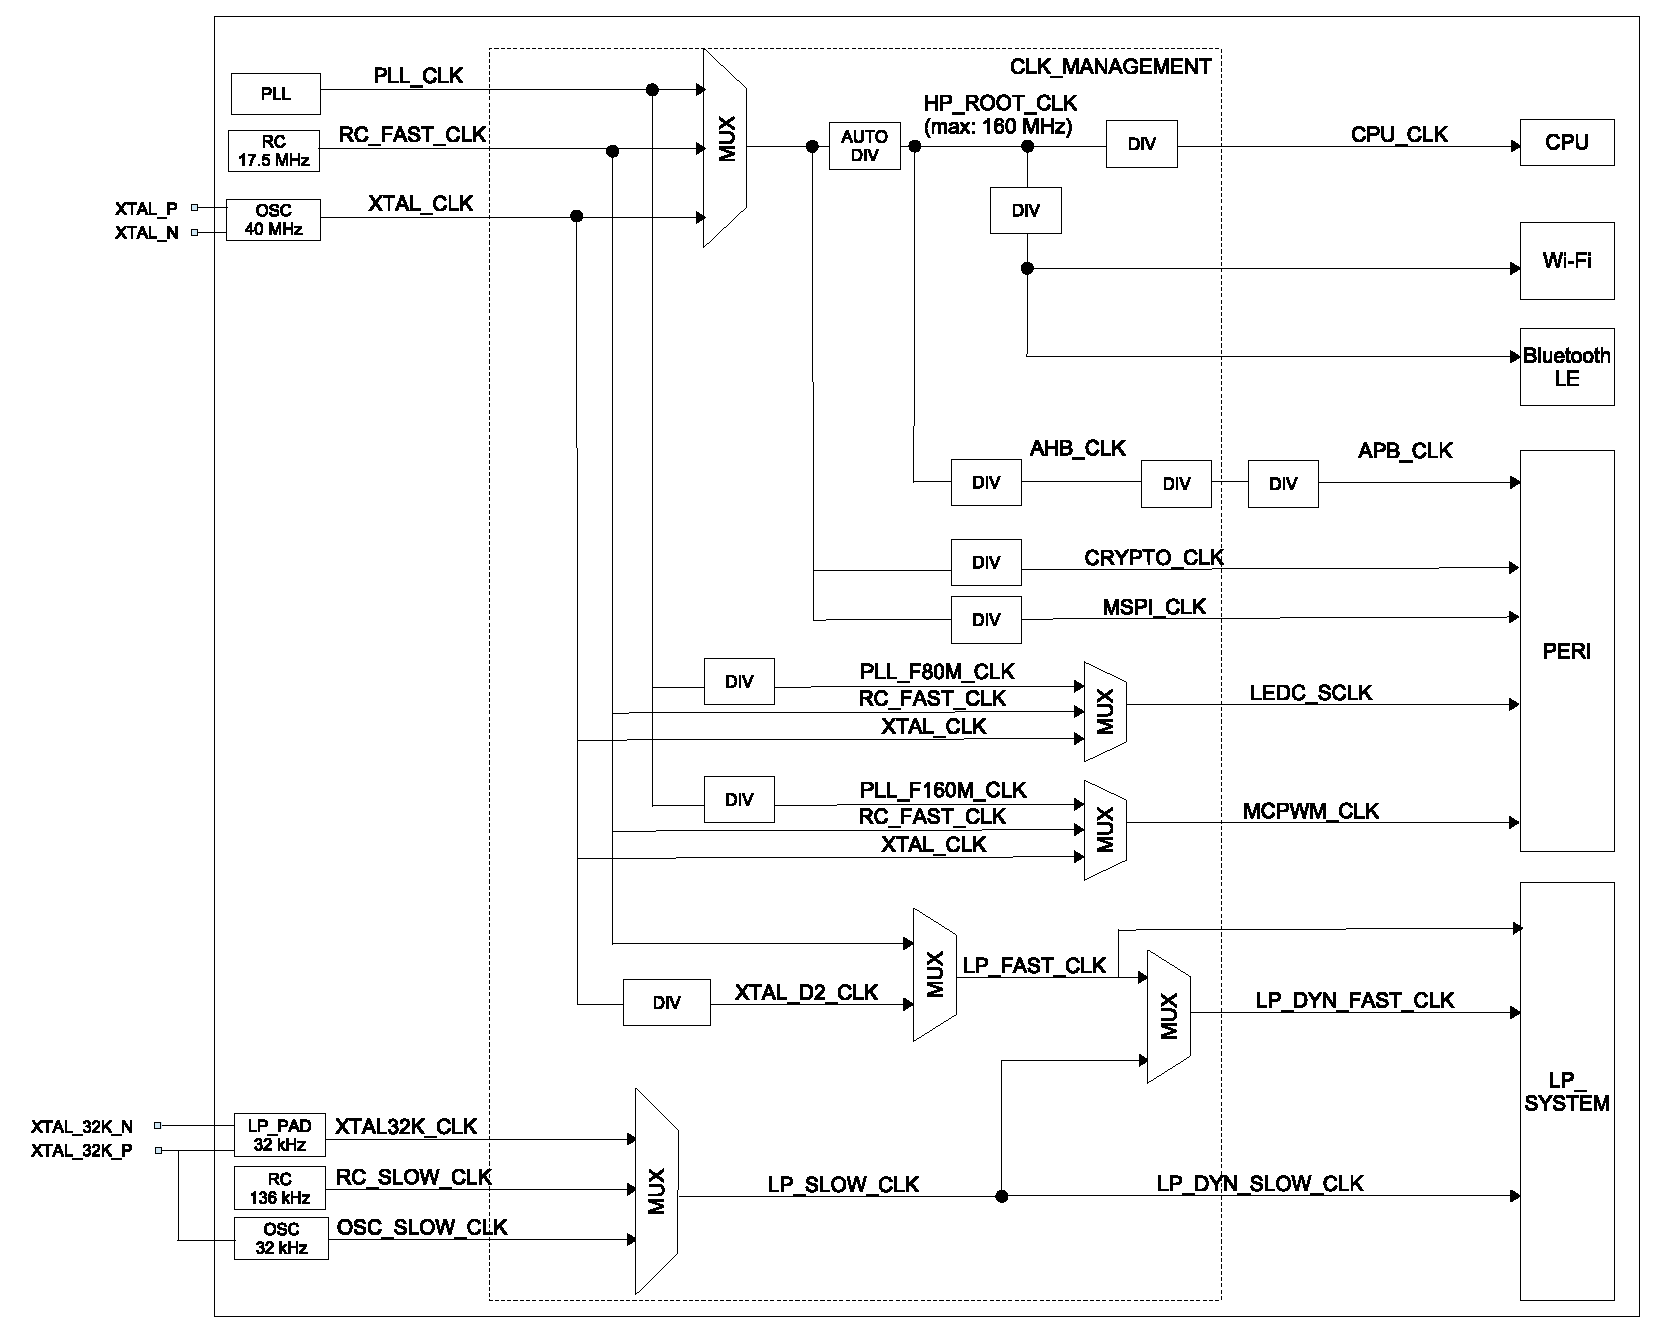
\includegraphics[width=1.0\textwidth]{./09-RESCLK/figures/sys_clk_struct.eps}
    \caption{系统时钟}
    \label{figure:Clock}
\end{figure}

\begin{tiplisting}
图中 AUTODIV 仅当前级 MUX 选择 PLL\_CLK 时，会由硬件控制将 480 MHz PLL\_CLK 分频为 160 MHz 时钟。若前级 MUX 选择 RC\_FAST\_CLK 或者 XTAL\_CLK 时，AUTODIV 不会对时钟分频。
\end{tiplisting}


\subsection{特性}

\chipname{} 的时钟源（见图 \ref{figure:Clock} 左侧）根据频率不同，可分为：
\begin{itemize}
    \item 高速时钟源，主要为 CPU 和数字外设提供工作时钟
    \begin{itemize}
        \item PLL\_CLK：480 MHz 内部 PLL 时钟（参考时钟是 XTAL\_CLK）
        \item XTAL\_CLK：40 MHz 外部晶振时钟
    \end{itemize}
    \item 低速时钟源，主要为低功耗系统以及部分处于低功耗模式的外设提供工作时钟
    \begin{itemize}
        \item XTAL32K\_CLK：32 kHz 外部晶振时钟
	    \item RC\_FAST\_CLK：内置快速 RC 振荡器时钟，频率可调节（通常为 17.5 MHz）
	    \item RC\_SLOW\_CLK：136 kHz 内置慢速 RC 振荡器
	    \item OSC\_SLOW\_CLK：外置低速时钟，通常频率为 32 kHz，通过 \hyperref[tab:iomuxgpio-iomax-pins-analog-functions]{XTAL\_32K\_P} 输入，在配置好这个 GPIO 的状态后需要配置 Hold 功能，具体请参考章节 \ref{mod:iomuxgpio} \textit{\nameref{mod:iomuxgpio}} >  \ref{PadHold} \textit{\nameref{PadHold}}
    \end{itemize}
\end{itemize}



\subsection{功能描述}

\subsubsection{高性能系统时钟}

如图 \ref{figure:Clock} 所示，CPU\_CLK 为 CPU 主时钟。CPU 在最高效工作模式下，主频可以达到 160 MHz。同时，CPU 能够在超低频下工作（通常为 2 MHz），以减少功耗。CPU\_CLK 与 AHB\_CLK、CRYPTO\_CLK、MSPI\_CLK 共用一个时钟源。用户可配置 \hyperref[fielddesc:PCRSOCCLKSEL]{PCR\_SOC\_CLK\_SEL} 选择 XTAL\_CLK、PLL\_CLK、或 RC\_FAST\_CLK 作为 CPU\_CLK 的时钟源，具体请参考表 \ref{tab:resclk-cpu-clk-src} 和表 \ref{tab:resclk-cpu-clk-freq}。当选择 PLL\_CLK 作为时钟源时，CPU\_CLK 会由硬件控制分频为 160 MHz 时钟（在配置分频器之前），可参考图 \ref{figure:Clock} 中的 AUTODIV。默认状态下，CPU 的时钟源为 XTAL\_CLK，且分频系数为 1 分频，即 40 MHz。

\begin{longtable}[c]{|p{5cm}|p{5cm}| }
       \caption{CPU\_CLK 时钟源选择}
		\label{tab:resclk-cpu-clk-src} \\
	    \hline
        \rowcolor{lightgray}
        \textbf{\hyperref[fielddesc:PCRSOCCLKSEL]{PCR\_SOC\_CLK\_SEL}} & \textbf{时钟源} \\
        \hline
        0 & XTAL\_CLK \\
        \hline
        1 & PLL\_CLK \\
        \hline
        2 & RC\_FAST\_CLK \\
        \hline
\end{longtable}

\begin{table}[H]
    \centering
    \caption{CPU\_CLK、AHB\_CLK 和 HP\_ROOT\_CLK 的时钟频率}
    \label{tab:resclk-cpu-clk-freq}

    \begin{threeparttable}
    \begin{tabular}{ |p{2.3cm}|p{4.0cm}|p{7.7cm}|}
    \hline
        \rowcolor{lightgray}
        \textbf{时钟名称} & \textbf{时钟源} & \textbf{时钟频率}\\\hline
		\multirow{3}{*} {HP\_ROOT\_CLK\tnote{1}} & PLL\_CLK & 480 MHz，会被硬件分频为 160 MHz 时钟 \\\cline{2-3}
		& XTAL\_CLK & 40 MHz \\\cline{2-3}
		& RC\_FAST\_CLK & 17.5 MHz\\\hline
		\multirow{2}{*} {CPU\_CLK\tnote{2}} & PLL\_CLK &  $f_{\textrm{HP\_ROOT\_CLK}}$/(\hyperref[fielddesc:PCRCPUHSDIVNUM]{PCR\_CPU\_HS\_DIV\_NUM} + 1) \\\cline{2-3}
		& {低速时钟源\tnote{3}} & $f_{\textrm{HP\_ROOT\_CLK}}$/(\hyperref[fielddesc:PCRCPULSDIVNUM]{PCR\_CPU\_LS\_DIV\_NUM} + 1)\\\hline
		\multirow{2}{*} {AHB\_CLK\tnote{4}} & PLL\_CLK & $f_{\textrm{HP\_ROOT\_CLK}}$/(\hyperref[fielddesc:PCRAHBHSDIVNUM]{PCR\_AHB\_HS\_DIV\_NUM} + 1) \\\cline{2-3}
		& 低速时钟源 & $f_{\textrm{HP\_ROOT\_CLK}}$/(\hyperref[fielddesc:PCRAHBLSDIVNUM]{PCR\_AHB\_LS\_DIV\_NUM} + 1)\\\hline

    \end{tabular}

        \begin{tablenotes}
            \item[1] HP\_ROOT\_CLK：经过选源后的 CPU\_CLK、AHB\_CLK、APB\_CLK 时钟源。若其时钟源为 PLL\_CLK，则会在选源后由硬件控制分频为 160 MHz 时钟
            \item[2] CPU 时钟频率应为 AHB 时钟频率的整数倍
            \item[3] 即 XTAL\_CLK 和 RC\_FAST\_CLK
            \item[4] AHB 时钟频率不能超过 40 MHz
        \end{tablenotes}
     \end{threeparttable}
    \end{table}


CPU\_CLK 和 AHB\_CLK 可选分频寄存器配置值如下（以十进制表述）：



\begin{itemize}
    \item \hyperref[fielddesc:PCRCPUHSDIVNUM]{PCR\_CPU\_HS\_DIV\_NUM} 可选值：0，1，3
    \item \hyperref[fielddesc:PCRCPULSDIVNUM]{PCR\_CPU\_LS\_DIV\_NUM} 可选值：0，1，3，7，15，31
    \item \hyperref[fielddesc:PCRAHBHSDIVNUM]{PCR\_AHB\_HS\_DIV\_NUM} 可选值：3，7，15
    \item \hyperref[fielddesc:PCRAHBLSDIVNUM]{PCR\_AHB\_LS\_DIV\_NUM} 可选值：0，1，3，7，15，31
\end{itemize}


如图 \ref{figure:Clock} 所示，APB\_CLK 是在 AHB\_CLK 基础上经过两级分频得到的。其中第一级分频为恒定分频，即始终按照分频系数 (\hyperref[fielddesc:PCRAPBDIVNUM]{PCR\_APB\_DIV\_NUM} + 1) 的值进行分频。第二级分频为自动降频，如果芯片中的主机没有访问外设寄存器的请求时，会以分频系数 (\hyperref[fielddesc:PCRAPBDECREASEDIVNUM]{APB\_DECREASE\_DIV\_NUM} + 1) 进行二次分频产生 APB\_CLK，但当芯片中的主机发起了访问外设寄存器的请求时，APB\_CLK 将恢复至一级分频后的频率。\\
注意，使用自动降频功能将降低芯片性能，用户可将 \hyperref[fielddesc:PCRAPBDECREASEDIVNUM]{APB\_DECREASE\_DIV\_NUM} 设置为 0 以禁用此功能。默认情况下，该功能禁用。

\subsubsection{低功耗系统时钟}

低功耗系统能够在大多数时钟源关闭的状态下工作。低功耗系统时钟包括 LP\_SLOW\_CLK 时钟和 LP\_FAST\_CLK 时钟。

LP\_SLOW\_CLK 和 LP\_FAST\_CLK 的时钟源为低频时钟，其中：
\begin{itemize}
    \item LP\_SLOW\_CLK 时钟有以下几种可能的时钟源：
    \begin{itemize}
        \item RC\_SLOW\_CLK
        \item XTAL32K\_CLK
        \item OSC\_SLOW\_CLK
    \end{itemize}
    \item LP\_FAST\_CLK 时钟有两种可能的时钟源：
    \begin{itemize}
        \item XTAL\_CLK 的 2 分频时钟 XTAL\_D2\_CLK (20 MHz)
        \item RC\_FAST\_CLK
    \end{itemize}
\end{itemize}

LP\_DYN\_SLOW\_CLK 时钟源为 LP\_SLOW\_CLK。

LP\_DYN\_FAST\_CLK 根据芯片电源的模式（详见章节 \ref{mod:lowpowm} \textit{\nameref{mod:lowpowm}}）选择时钟源：

\begin{itemize}
    \item 芯片电源为 Active、Modem-sleep 模式时始终选择 LP\_FAST\_CLK 作为时钟源
    \item 芯片电源为 Light-sleep、Deep-sleep 模式时选择 LP\_SLOW\_CLK 作为时钟源
\end{itemize}

\subsubsection{外设时钟}
表 \ref{tab:resclk-periph-clks-root}、表 \ref{tab:resclk-periph-clks-hp} 和表 \ref{tab:resclk-periph-clks-lp} 分别列出了接入各个外设时钟的衍生时钟源、接入高性能系统各个外设的时钟以及接入低功耗系统各个外设时钟。




\begin{landscape}


\begin{tiny}
\begin{longtable}[c]{|p{1.4cm}|C{0.67cm}|C{0.2cm}|C{0.2cm}|C{0.2cm}|C{0.19cm}|C{0.19cm}|C{0.7cm}|C{0.8cm}|C{1.2cm}|C{0.7cm}|C{1.1cm}|C{0.7cm}|C{1.0cm}|C{0.7cm}|C{0.7cm}|C{0.7cm}|C{0.9cm}|C{0.9cm}|C{0.9cm}|C{1.0cm}|C{1.3cm}| }

 \caption{衍生时钟源}
    \label{tab:resclk-periph-clks-root} \\
  \hline
    \rowcolor{lightgray}
        & \multicolumn{2}{c|}{\textbf{Source Clock}} & \multicolumn{4}{c|}{\textbf{Derived Clock}} & \multicolumn{4}{c|}{\textbf{Source Clock}} & \multicolumn{10}{c|}{\textbf{Derived Clock}}  &  \textbf{Source Clock}\\\cline{2-22}
        \rowcolor{lightgray}
        & \textbf{XTAL\_CLK} & \multicolumn{5}{c|}{\textbf{PLL\_CLK}} & \textbf{RC\_FAST\_} & \textbf{RC\_SLOW\_}& &\textbf{XTAL32K\_} &\textbf{HP\_ROOT\_CLK} & & & & & & \textbf{LP\_DYN\_}& \textbf{LP\_DYN\_}&\textbf{XTAL\_D2\_CLK} & & \\\cline{3-7}
        \rowcolor{lightgray}
        \multirow{-3}{*}{\textbf{Derived Clock}} & \textbf{40 MHz} & \textbf{480 MHz} & \textbf{240 MHz} & \textbf{160 MHz} & \textbf{80 MHz} & \textbf{48 MHz} & \textbf{CLK 17.5 MHz} & \textbf{CLK 136 kHz} & \textbf{OSC\_SLOW\_CLK 32 kHz} & \textbf{CLK 32 kHz} & \textbf{160 MHz/40 MHz/17.5 MHz} & \multirow{-2}{*}{\textbf{MSPI\_CLK}} & \multirow{-2}{*}{\textbf{CRYPTO\_CLK}} & \multirow{-2}{*}{\textbf{APB\_CLK}} & \multirow{-2}{*}{\textbf{AHB\_CLK}} & \multirow{-2}{*}{\textbf{CPU\_CLK}} & \multirow{-2}{*}{\textbf{FAST\_CLK}} & \multirow{-2}{*}{\textbf{SLOW\_CLK}} & \textbf{20 MHz} & \multirow{-2}{*}{\textbf{LP\_FAST\_CLK}} & \multirow{-2}{*}{\textbf{CLOCK FROM IO}}
        \\\hline
        \endfirsthead

    \multicolumn{22}{c}{\bfseries \tablename\ \thetable{} -- 接上页}\\\hline
    \rowcolor{lightgray}
        & \multicolumn{2}{c|}{\textbf{Source Clock}} & \multicolumn{4}{c|}{\textbf{Derived Clock}} & \multicolumn{4}{c|}{\textbf{Source Clock}} & \multicolumn{10}{c|}{\textbf{Derived Clock}}  &  \textbf{Source Clock}\\\cline{2-22}
        \rowcolor{lightgray}
        & \textbf{XTAL\_CLK} & \multicolumn{5}{c|}{\textbf{PLL\_CLK}} & \textbf{RC\_FAST\_} & \textbf{RC\_SLOW\_}&  &\textbf{XTAL32K\_} &\textbf{HP\_ROOT\_CLK} & & & & & & \textbf{LP\_DYN\_}& \textbf{LP\_DYN\_}&\textbf{XTAL\_D2\_CLK} & & \\\cline{3-7}
        \rowcolor{lightgray}
        \multirow{-3}{*}{\textbf{Derived Clock}} & \textbf{40 MHz} & \textbf{480 MHz} & \textbf{240 MHz} & \textbf{160 MHz} & \textbf{80 MHz} & \textbf{48 MHz} & \textbf{CLK 17.5 MHz} & \textbf{CLK 136 kHz} & \textbf{OSC\_SLOW\_CLK 32 kHz} & \textbf{CLK 32 kHz} & \textbf{160 MHz/40 MHz/17.5 MHz} & \multirow{-2}{*}{\textbf{MSPI\_CLK}} & \multirow{-2}{*}{\textbf{CRYPTO\_CLK}} & \multirow{-2}{*}{\textbf{APB\_CLK}} & \multirow{-2}{*}{\textbf{AHB\_CLK}} & \multirow{-2}{*}{\textbf{CPU\_CLK}} & \multirow{-2}{*}{\textbf{FAST\_CLK}} & \multirow{-2}{*}{\textbf{SLOW\_CLK}} & \textbf{20 MHz} & \multirow{-2}{*}{\textbf{LP\_FAST\_CLK}} & \multirow{-2}{*}{\textbf{CLOCK FROM IO}}\\\hline
    \endhead

    \multicolumn{22}{r}{\textbf{见下页}} \\
    \endfoot
    \endlastfoot
    \hline

PLL\_48M $\sim$ 240M\_CLK & & Y & & & & & & & & & & & & & & & & & & &  \\\hline
HP\_ROOT\_CLK & Y& Y & & & & & Y & & & & & & & & & & & & & &  \\\hline
MSPI\_CLK & & & & & & & & & & & Y & & & & & & & & & &  \\\hline
CRYPTO\_CLK & & & & & & & & & & & Y & & & & & & & & & &  \\\hline
APB\_CLK& & & & & & & & & & & Y & & & & & & & & & &  \\\hline
AHB\_CLK& & & & & & & & & & & Y & & & & & & & & & &  \\\hline
CPU\_CLK & & & & & & & & & & & Y & & & & & & & & & &  \\\hline
LP\_DYN\_FAST\_CLK& & & & & & &  & Y & Y & Y & & & & & & & & &  & Y &  \\\hline
LP\_DYN\_SLOW\_CLK& & & & & & &  & Y & Y & Y & & & & & & & & &  & & \\\hline
XTAL\_D2\_CLK & Y & & & & & & & & & & & & & & & & & & & &  \\\hline
LP\_FAST\_CLK & & & & & & & Y & & & & & & & & & & & & Y & &  \\\hline
\end{longtable}

\begin{longtable}[c]{|p{1.4cm}|C{0.67cm}|C{0.2cm}|C{0.2cm}|C{0.2cm}|C{0.19cm}|C{0.19cm}|C{0.7cm}|C{0.8cm}|C{1.2cm}|C{0.7cm}|C{1.1cm}|C{0.7cm}|C{1.0cm}|C{0.7cm}|C{0.7cm}|C{0.7cm}|C{0.9cm}|C{0.9cm}|C{0.9cm}|C{1.0cm}|C{1.3cm}| }

 \caption{高性能系统外设时钟}
    \label{tab:resclk-periph-clks-hp} \\
  \hline
    \rowcolor{lightgray}
        & \multicolumn{2}{c|}{\textbf{Source Clock}} & \multicolumn{4}{c|}{\textbf{Derived Clock}} & \multicolumn{4}{c|}{\textbf{Source Clock}} & \multicolumn{10}{c|}{\textbf{Derived Clock}}  &  \textbf{Source Clock}\\\cline{2-22}
        \rowcolor{lightgray}
        & \textbf{XTAL\_CLK} & \multicolumn{5}{c|}{\textbf{PLL\_CLK}} & \textbf{RC\_FAST\_} & \textbf{RC\_SLOW\_}& & \textbf{XTAL32K\_} &\textbf{HP\_ROOT\_CLK} & & & & & &\textbf{LP\_DYN\_} &\textbf{LP\_DYN\_} &\textbf{XTAL\_D2\_CK} & & \\\cline{3-7}
        \rowcolor{lightgray}
        \multirow{-3}{*}{\textbf{Peripheral}} & \textbf{40 MHz} & \textbf{480 MHz} & \textbf{240 MHz} & \textbf{160 MHz} & \textbf{80 MHz} & \textbf{48 MHz} & \textbf{CLK 17.5 MHz} & \textbf{CLK 136 kHz} & \textbf{OSC\_SLOW\_CLK 32 kHz} & \textbf{CLK 32 kHz} & \textbf{160 MHz/40 MHz/17.5 MHz} & \multirow{-2}{*}{\textbf{MSPI\_CLK}} & \multirow{-2}{*}{\textbf{CRYPTO\_CLK}} & \multirow{-2}{*}{\textbf{APB\_CLK}} & \multirow{-2}{*}{\textbf{AHB\_CLK}} & \multirow{-2}{*}{\textbf{CPU\_CLK}} & \textbf{FAST\_CLK} & \textbf{SLOW\_CLK} & \textbf{20 MHz} & \multirow{-2}{*}{\textbf{LP\_FAST\_CLK}} & \multirow{-2}{*}{\textbf{CLOCK FROM IO}}
        \\\hline
        \endfirsthead

    \multicolumn{22}{c}{\bfseries \tablename\ \thetable{} -- 接上页}\\\hline
    \rowcolor{lightgray}
        & \multicolumn{2}{c|}{\textbf{Source Clock}} & \multicolumn{4}{c|}{\textbf{Derived Clock}} & \multicolumn{4}{c|}{\textbf{Source Clock}} & \multicolumn{10}{c|}{\textbf{Derived Clock}}  &  \textbf{Source Clock}\\\cline{2-22}
        \rowcolor{lightgray}
        & \textbf{XTAL\_CLK} & \multicolumn{5}{c|}{\textbf{PLL\_CLK}} & \textbf{RC\_FAST\_} & \textbf{RC\_SLOW\_}& & \textbf{XTAL32K\_} &\textbf{HP\_ROOT\_CLK} & & & & & &\textbf{LP\_DYN\_} &\textbf{LP\_DYN\_} &\textbf{XTAL\_D2\_CK} & & \\\cline{3-7}
        \rowcolor{lightgray}
        \multirow{-3}{*}{\textbf{Peripheral}} & \textbf{40 MHz} & \textbf{480 MHz} & \textbf{240 MHz} & \textbf{160 MHz} & \textbf{80 MHz} & \textbf{48 MHz} & \textbf{CLK 17.5 MHz} & \textbf{CLK 136 kHz} & \textbf{OSC\_SLOW\_CLK 32 kHz} & \textbf{CLK 32 kHz} & \textbf{160 MHz/40 MHz/17.5 MHz} & \multirow{-2}{*}{\textbf{MSPI\_CLK}} & \multirow{-2}{*}{\textbf{CRYPTO\_CLK}} & \multirow{-2}{*}{\textbf{APB\_CLK}} & \multirow{-2}{*}{\textbf{AHB\_CLK}} & \multirow{-2}{*}{\textbf{CPU\_CLK}} & \textbf{FAST\_CLK} & \textbf{SLOW\_CLK} & \textbf{20 MHz} & \multirow{-2}{*}{\textbf{LP\_FAST\_CLK}} & \multirow{-2}{*}{\textbf{CLOCK FROM IO}}\\\hline
    \endhead

    \multicolumn{22}{r}{\textbf{见下页}} \\
    \endfoot
    \endlastfoot
    \hline

\nameref{mod:timg} & Y & & & & Y & & Y & & & & & & & & & & & & & &  \\\hline
\hyperref[mod:wdt]{主系统看门狗定时器 (MWDT)} & Y & & & & Y & & Y & & & & & & & & & & & & & &  \\\hline
\nameref{mod:i2s} & Y & & Y & Y & & & & & & & & & & & & & & & & & I2S\_MCLK\_PAD  \\\hline
\hyperref[mod:uart]{UART 控制器 (UART)} & Y & & & & Y & & Y & & & & & & & & & & & & & &  \\\hline
\nameref{mod:rmt} & Y & & & & Y & & Y & & & & & & & & & & & & & &  \\\hline
\nameref{mod:mcpwm} & Y & & & Y & & & Y & & & & & & & & & & & & & &  \\\hline
\nameref{mod:i2c}  & Y & & & & & & Y & & & & & & & & & & & & & &  \\\hline
\hyperref[mod:spi]{SPI2} & Y & & & & Y & & Y & & & & & & & & & & & & & &  \\\hline
\hyperref[mod:sensor]{SAR ADC} & Y & &  & & Y & & Y & & & & & & & & & & & & & &  \\\hline
\nameref{mod:usbserialjtag} & & & & & & Y & & & & & & & & & & & & & & &  \\\hline
\nameref{mod:twai} & Y & & & & & & Y & & & & & & & & & & & & & &  \\\hline
\nameref{mod:ledpwm} & Y & & & & Y & & Y & & & & & & & & & & & & & &  \\\hline
\nameref{mod:systimer} & Y & & & & & & Y & & & & & & & & & & & & & &  \\\hline
\nameref{mod:parlio} & Y & & Y & & & & Y & & & & & & & & & & & & & & PARL\_CLK\_PAD \\\hline
\hyperref[mod:iomuxgpio]{IO MUX} & Y & & & & Y & & Y & & & & & & & & & & & & & &  \\\hline
\nameref{mod:aes}/\nameref{mod:sha}/\nameref{mod:rsa}/\nameref{mod:ecc}/\nameref{mod:digsig}/\nameref{mod:hmac} & & & & & & & & & & & & & Y & & & & & & & &  \\\hline
\nameref{mod:intmtrx} & & & & & & & & & & & & & & & Y & & & & & &  \\\hline
\nameref{mod:pcnt} & & & & & & & & & & & & & & Y & & & & & & &  \\\hline
\nameref{mod:evntaskmatrix} & & & & & & & & & & & & & & & Y & & & & & & \\\hline
\nameref{mod:dma} & & & & & & & & & & & & & & & Y & & & & & & \\\hline
\hyperref[mod:uart]{UHCI} & & & & & & & & & & & & & & & Y & & & & & & \\\hline
\end{longtable}


\begin{longtable}[c]{|p{1.4cm}|C{0.67cm}|C{0.2cm}|C{0.2cm}|C{0.2cm}|C{0.19cm}|C{0.19cm}|C{0.7cm}|C{0.8cm}|C{1.2cm}|C{0.7cm}|C{1.1cm}|C{0.7cm}|C{1.0cm}|C{0.7cm}|C{0.7cm}|C{0.7cm}|C{0.9cm}|C{0.9cm}|C{0.9cm}|C{1.0cm}|C{1.3cm}| }

 \caption{低功耗系统外设时钟}
    \label{tab:resclk-periph-clks-lp} \\
  \hline
    \rowcolor{lightgray}
        & \multicolumn{2}{c|}{\textbf{Source Clock}} & \multicolumn{4}{c|}{\textbf{Derived Clock}} & \multicolumn{4}{c|}{\textbf{Source Clock}} & \multicolumn{10}{c|}{\textbf{Derived Clock}}  &  \textbf{Source Clock}\\\cline{2-22}
        \rowcolor{lightgray}
        & \textbf{XTAL\_CLK} & \multicolumn{5}{c|}{\textbf{PLL\_CLK}} & \textbf{RC\_FAST\_} & \textbf{RC\_SLOW\_}& & \textbf{XTAL32K\_} &\textbf{HP\_ROOT\_CLK} & & & & & &\textbf{LP\_DYN\_} &\textbf{LP\_DYN\_} &\textbf{XTAL\_D2\_CK} & & \\\cline{3-7}
        \rowcolor{lightgray}
        \multirow{-3}{*}{\textbf{Peripheral}} & \textbf{40 MHz} & \textbf{480 MHz} & \textbf{240 MHz} & \textbf{160 MHz} & \textbf{80 MHz} & \textbf{48 MHz} & \textbf{CLK 17.5 MHz} & \textbf{CLK 136 kHz} & \textbf{OSC\_SLOW\_CLK 32 kHz} & \textbf{CLK 32 kHz} & \textbf{160 MHz/40 MHz/17.5 MHz} & \multirow{-2}{*}{\textbf{MSPI\_CLK}} & \multirow{-2}{*}{\textbf{CRYPTO\_CLK}} & \multirow{-2}{*}{\textbf{APB\_CLK}} & \multirow{-2}{*}{\textbf{AHB\_CLK}} & \multirow{-2}{*}{\textbf{CPU\_CLK}} & \textbf{FAST\_CLK} & \textbf{SLOW\_CLK} & \textbf{20 MHz} & \multirow{-2}{*}{\textbf{LP\_FAST\_CLK}} & \multirow{-2}{*}{\textbf{CLOCK FROM IO}}
        \\\hline
        \endfirsthead

    \multicolumn{22}{c}{\bfseries \tablename\ \thetable{} -- 接上页}\\\hline
    \rowcolor{lightgray}
        & \multicolumn{2}{c|}{\textbf{Source Clock}} & \multicolumn{4}{c|}{\textbf{Derived Clock}} & \multicolumn{4}{c|}{\textbf{Source Clock}} & \multicolumn{10}{c|}{\textbf{Derived Clock}}  &  \textbf{Source Clock}\\\cline{2-22}
        \rowcolor{lightgray}
        & \textbf{XTAL\_CLK} & \multicolumn{5}{c|}{\textbf{PLL\_CLK}} & \textbf{RC\_FAST\_} & \textbf{RC\_SLOW\_}& & \textbf{XTAL32K\_} &\textbf{HP\_ROOT\_CLK} & & & & & &\textbf{LP\_DYN\_} &\textbf{LP\_DYN\_} &\textbf{XTAL\_D2\_CK} & & \\\cline{3-7}
        \rowcolor{lightgray}
        \multirow{-3}{*}{\textbf{Peripheral}} & \textbf{40 MHz} & \textbf{480 MHz} & \textbf{240 MHz} & \textbf{160 MHz} & \textbf{80 MHz} & \textbf{48 MHz} & \textbf{CLK 17.5 MHz} & \textbf{CLK 136 kHz} & \textbf{OSC\_SLOW\_CLK 32 kHz} & \textbf{CLK 32 kHz} & \textbf{160 MHz/40 MHz/17.5 MHz} & \multirow{-2}{*}{\textbf{MSPI\_CLK}} & \multirow{-2}{*}{\textbf{CRYPTO\_CLK}} & \multirow{-2}{*}{\textbf{APB\_CLK}} & \multirow{-2}{*}{\textbf{AHB\_CLK}} & \multirow{-2}{*}{\textbf{CPU\_CLK}} & \textbf{FAST\_CLK} & \textbf{SLOW\_CLK} & \textbf{20 MHz} & \multirow{-2}{*}{\textbf{LP\_FAST\_CLK}} & \multirow{-2}{*}{\textbf{CLOCK FROM IO}}\\\hline
    \endhead

    \multicolumn{22}{r}{\textbf{见下页}} \\
    \endfoot
    \endlastfoot
    \hline

\hyperref[mod:efuse]{eFuse 控制器 (eFuse)} & & & & & & & & & & & & & & & & & & & Y & &  \\\hline
\hyperref[mod:wdt]{RTC 看门狗定时器 (RWDT)} & & & & & & & & & & & & & & & & & Y & Y & & &  \\\hline
RTC 定时器 (RTC Timer) & & & & & & & & & & & & & & & & & Y & Y & & &  \\\hline
欠压检测器 (Brownout Detector) & & & & & & & & & & & & & & & & & Y & & & &  \\\hline
电源管理单元 (PMU) & & & & & & & & & & & & & & & & & Y & Y & & Y &  \\\hline
\hyperref[mod:uart]{UART 控制器 (LP\_UART)} & & & & & & & & & & & & & & & & & & & Y & Y &  \\\hline
\nameref{mod:ulp} & & & & & & & & & & & & & & & & & & & & Y &  \\\hline
\hyperref[mod:i2c]{I2C 控制器 (LP\_I2C)} & & & & & & & & & & & & & & & & & & & Y & Y &  \\\hline
\hyperref[mod:iomuxgpio]{LP\_IO MUX} & & & & & & & & & & & & & & & & & Y & & & &  \\\hline
\end{longtable}
\end{tiny}

\end{landscape}


\textbf{PLL\_CLK 时钟}

PLL\_F480M\_CLK 是 PLL 的源时钟，为 480 MHz 。PLL\_D2\_CLK (240 MHz)、PLL\_F160M\_CLK、PLL\_F80M\_CLK、PLL\_F48M\_CLK 均为 PLL\_F480M\_CLK 分频所得。

\textbf{CRYPTO\_CLK 时钟}

如图 \ref{figure:Clock} 所示，CRYPTO\_CLK 时钟的时钟源与 CPU\_CLK 相同，CRYPTO\_CLK 时钟频率最大为 160 MHz。


为了防止 DPA (Differential Power Analysis) 攻击加解密外设，加解密功能时钟采用随机分频策略。根据随机分频范围划分为四个安全等级。可通过配置 \hyperref[regdesc:HPSYSTEMSECDPACONFREG]{HP\_SYSTEM\_SEC\_DPA\_CONF\_REG} 选择安全等级。当 \hyperref[fielddesc:HPSYSTEMSECDPACFGSEL]{HP\_SYSTEM\_SEC\_DPA\_CFG\_SEL} 为 1 时，安全等级由 eFuse 中的配置信息 (\hyperref[fielddesc:EFUSESECDPALEVEL]{EFUSE\_SEC\_DPA\_LEVEL}) 决定，否则由 \hyperref[fielddesc:HPSYSTEMSECDPALEVEL]{HP\_SYSTEM\_SEC\_DPA\_LEVEL} 的值决定。


\textbf{LED\_PWM 时钟}


LEDC 模块能将 PLL\_F80M\_CLK、RC\_FAST\_CLK 以及 XTAL\_CLK 作为时钟源使用，即在 APB\_CLK 关闭的时候，LEDC 也可工作。换而言之，当系统处于低功耗模式时，其它外设都将停止工作（APB\_CLK 关闭），但是 LEDC 仍然可以通过 RC\_FAST\_CLK 来正常工作。

\subsubsection{Wi-Fi 和 Bluetooth LE 时钟}

Wi-Fi 和 Bluetooth LE 必须在 CPU\_CLK 时钟源选择 PLL\_CLK 下才能工作。只有当 Wi-Fi 和 Bluetooth LE 进入低功耗模式时，才能暂时关闭 PLL\_CLK。

\subsection{PMU 控制高性能系统时钟门控}

在 \chipname{} 的各个工作模式下，可提前配置以下寄存器字段，实现 PMU 对高性能系统外设的时钟门控：
\begin{itemize}
    \item \hyperref[fielddesc:PMUHPACTIVEDIGICGAPBEN]{PMU\_HP\_\regindex{x}\_DIG\_ICG\_APB\_EN} (x = ACTIVE/MODEM/SLEEP)：控制高性能系统外设读写寄存器的时钟门控
    \item \hyperref[fielddesc:PMUHPACTIVEDIGICGFUNCEN]{PMU\_HP\_\regindex{x}\_DIG\_ICG\_FUNC\_EN} (x = ACTIVE/MODEM/SLEEP)：控制高性能系统外设的工作时钟门控。
\end{itemize}

具体配置流程请参考章节 \ref{mod:lowpowm} \textit{\nameref{mod:lowpowm}}。

表 \ref{tab:clk_pmu_apb} 和表 \ref{tab:clk_pmu_func} 列出了 PMU 预配置寄存器位与高性能系统时钟门控的对应关系。


\begin{table}[H]
    \centering
    \caption{控制模块的读写寄存器时钟门控与 PMU 相关寄存器映射关系}\label{tab:clk_pmu_apb}
\begin{tabular}{|l|l|}
\hline
\rowcolor{lightgray}
\hyperref[fielddesc:PMUHPACTIVEDIGICGAPBEN]{PMU\_HP\_\regindex{x}\_DIG\_ICG\_APB\_EN} \textbf{位} & \textbf{控制模块的读写寄存器时钟门控} \\ \hline
0                                   &        \makecell[l]{\nameref{mod:aes}\\\nameref{mod:sha}\\\nameref{mod:rsa}\\\nameref{mod:ecc}\\\nameref{mod:digsig}\\\nameref{mod:hmac}}        \\ \hline
1                                   &      \nameref{mod:dma}          \\ \hline
2                                   &          \hyperref[mod:spi]{SPI2}      \\ \hline
3                                   &          \nameref{mod:intmtrx}      \\ \hline
4                                   &         \nameref{mod:i2s}       \\ \hline
6                                   &      \hyperref[mod:uart]{UART0}          \\ \hline
7                                   &       \hyperref[mod:uart]{UART1}         \\ \hline
8                                   &       \hyperref[mod:uart]{UHCI}         \\ \hline
11                                  &       \hyperref[mod:timg]{定时器组 0}         \\ \hline
12                                  &       \hyperref[mod:timg]{定时器组 1}         \\ \hline
13                                  &       \nameref{mod:i2c}         \\ \hline
14                                  &       \nameref{mod:ledpwm}         \\ \hline
15                                  &       \nameref{mod:rmt}         \\ \hline
16                                  &       \nameref{mod:systimer}         \\ \hline
17                                  &       \nameref{mod:usbserialjtag}         \\ \hline
18                                  &       \hyperref[mod:twai]{双线汽车接口 0}         \\ \hline
19                                  &       \hyperref[mod:twai]{双线汽车接口 1}         \\ \hline
20                                  &       \nameref{mod:pcnt}         \\ \hline
21                                  &       \nameref{mod:mcpwm}         \\ \hline
22                                  &       \nameref{mod:evntaskmatrix}         \\ \hline
23                                  &       \nameref{mod:parlio}         \\ \hline
25                                  &       \nameref{mod:dbgassist}         \\ \hline
26                                  &       \nameref{mod:iomuxgpio}         \\ \hline
\end{tabular}
\end{table}


\begin{table}[H]
    \centering
    \caption{控制模块的工作时钟门控与 PMU 相关寄存器映射关系}\label{tab:clk_pmu_func}
\begin{tabular}{|l|l|}
\hline
\rowcolor{lightgray}
\hyperref[fielddesc:PMUHPACTIVEDIGICGFUNCEN]{PMU\_HP\_\regindex{x}\_DIG\_ICG\_FUNC\_EN} \textbf{位} & \textbf{控制模块的功能时钟门控} \\ \hline
0                                   &    \nameref{mod:dma}            \\ \hline
1                                   &    \hyperref[mod:spi]{SPI2}            \\ \hline
2                                   &    \hyperref[mod:i2s]{I2S 接收侧}            \\ \hline
3                                   &    \hyperref[mod:uart]{UART0}            \\ \hline
4                                   &    \hyperref[mod:uart]{UART1}            \\ \hline
5                                   &    \hyperref[mod:uart]{UHCI}            \\ \hline
6                                   &    \nameref{mod:usbserialjtag}            \\ \hline
7                                   &    \hyperref[mod:i2s]{I2S 发送侧}            \\ \hline
10                                  &    \nameref{mod:dbgassist}            \\ \hline
11                                  &    \nameref{mod:sdioslave}            \\ \hline
12                                  &    \nameref{mod:sensor}            \\ \hline
13                                  &    \hyperref[mod:timg]{定时器组 0}            \\ \hline
14                                  &    \hyperref[mod:timg]{定时器组 1}            \\ \hline
16                                  &    \nameref{mod:evntaskmatrix}            \\ \hline
17                                  &    \nameref{mod:riscvcpu}            \\ \hline
18                                  &    \nameref{mod:systimer}            \\ \hline
19                                  &    \makecell[l]{\nameref{mod:aes}\\\nameref{mod:sha}\\\nameref{mod:rsa}\\\nameref{mod:ecc}\\\nameref{mod:digsig}\\\nameref{mod:hmac}}            \\ \hline
21                                  &    \nameref{mod:rmt}            \\ \hline
22                                  &    \nameref{mod:mcpwm}            \\ \hline
24                                  &    \hyperref[mod:parlio]{并行 IO 控制器发送侧}            \\ \hline
25                                  &    \hyperref[mod:parlio]{并行 IO 控制器接收侧}             \\ \hline
27                                  &     \nameref{mod:ledpwm}           \\ \hline
28                                  &     \nameref{mod:iomuxgpio}           \\ \hline
29                                  &     \nameref{mod:i2c}           \\ \hline
30                                  &       \hyperref[mod:twai]{双线汽车接口 0}         \\ \hline
31                                  &       \hyperref[mod:twai]{双线汽车接口 1}         \\ \hline
\end{tabular}
\end{table}



\section{配置流程}
\label{sec:alias-prog-procedures}

\subsection{高性能系统时钟配置}


可配置 \hyperref[fielddesc:PCRSOCCLKSEL]{PCR\_SOC\_CLK\_SEL} 选择 HP\_ROOT\_CLK 的时钟选源。


当 HP\_ROOT\_CLK 的时钟源为 PLL\_CLK 时，可配置 \hyperref[fielddesc:PCRCPUHSDIVNUM]{PCR\_CPU\_HS\_DIV\_NUM} 选择 CPU\_CLK 的时钟分频系数。可配置 \hyperref[fielddesc:PCRAHBHSDIVNUM]{PCR\_AHB\_HS\_DIV\_NUM} 选择 AHB\_CLK 的时钟分频系数。


当 HP\_ROOT\_CLK 的时钟源为 XTAL\_CLK 或 RC\_FAST\_CLK 时， 可配置 \hyperref[fielddesc:PCRCPULSDIVNUM]{PCR\_CPU\_LS\_DIV\_NUM} 选择 CPU\_CLK 的时钟分频系数。可配置 \hyperref[fielddesc:PCRAHBLSDIVNUM]{PCR\_AHB\_LS\_DIV\_NUM} 选择 AHB\_CLK 的时钟分频系数。

\subsection{低功耗系统时钟配置}

可配置 \hyperref[fielddesc:LPCLKRSTSLOWCLKSEL]{LP\_CLKRST\_SLOW\_CLK\_SEL} 选择 LP\_SLOW\_CLK 的时钟源。

可配置 \hyperref[fielddesc:LPCLKRSTFASTCLKSEL]{LP\_CLKRST\_FAST\_CLK\_SEL} 选择 LP\_FAST\_CLK 的时钟源。

\subsection{外设时钟复位配置}\label{sec:periperal-clock-configuration}

\begin{importantlisting}
\vspace{-0.5em}

\chipname{} 具有低功耗特性，因此有些外设时钟默认为关闭状态。在启用这些外设之前，必须将外设的时钟打开，即把相应的 CLK\_EN 位置为 1，并且解除外设的复位状态，即把相应的 RST\_EN 位置为 0。
\end{importantlisting}

大部分外设模块的时钟都可以分为总线时钟和功能时钟。外设寄存器的总线时钟主要是用于配置外设寄存器。功能时钟主要是模块工作所使用的时钟，例如 UART 的参考时钟。大部分模块的功能时钟可以选择多个时钟源。在门控寄存器的描述中会说明该寄存器属于总线（AHB\_CLK、APB\_CLK）时钟门控寄存器还是功能时钟门控寄存器。

\chipname{} 的总线时钟开关、功能时钟的开关以及时钟源选择和时钟分频的配置寄存器均放在了 PCR 模块中。功能模块不工作时，可以配置该寄存器关闭功能时钟，关闭模块功能时钟不会影响系统其他部分。

下文以 I2C 时钟配置为例：


\begin{figure}[H]
    \centering
    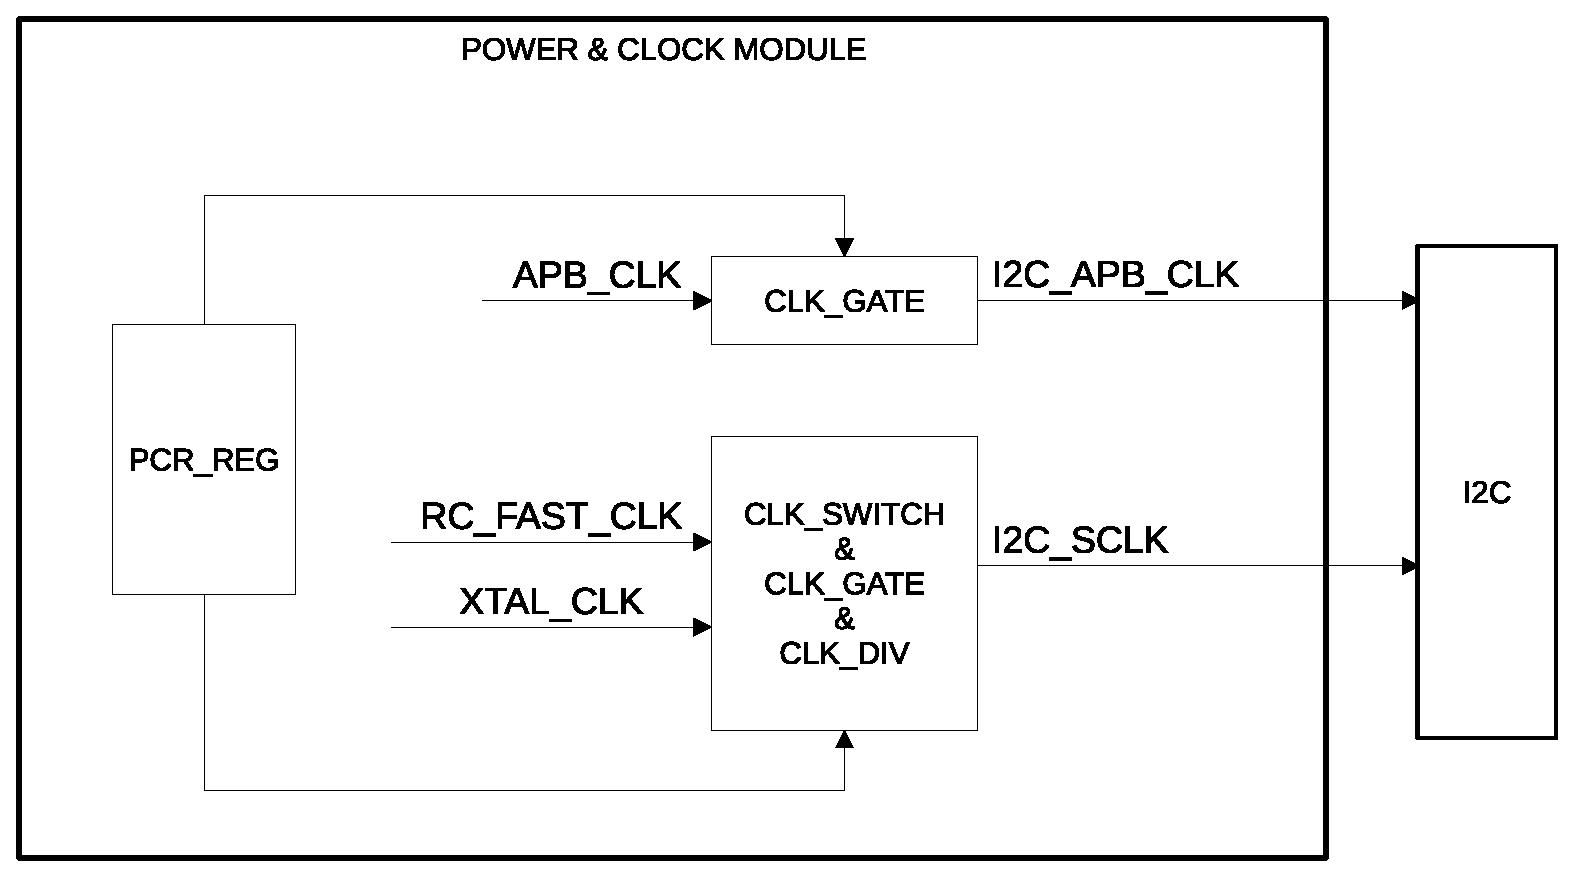
\includegraphics[width=1.0\textwidth]{./09-RESCLK/figures/sys_clk_struct_pcr.eps}
    \caption{时钟配置示例}
    \label{figure:Clock Config}
\end{figure}


图 \ref{figure:Clock Config} 是I2C的时钟结构图，其他模块的时钟结构类似。其中CLK\_SWITCH 的功能是选择一个时钟输出，CLK\_GATE 的功能是打开/关闭时钟。

对于要求低功耗的场景，当模块不工作时，除了关闭功能时钟，还可以关闭模块的总线时钟来进一步降低功耗。注意，如果先关闭模块总线时钟，那么模块的功能时钟还是有可能继续工作，所以推荐先关闭功能时钟再关闭总线时钟，打开时钟时推荐先打开总线时钟再打开功能时钟。




\hypertarget{resclk-reg-summ}{}
\section{寄存器列表}\label{sec:resclk-reg-summ}


\subsection{PCR 模块寄存器列表}


本小节的所有地址均为相对于电源/时钟/复位寄存器（PCR）基地址的地址偏移量（相对地址），具体基地址请见章节 \ref{mod:sysmem} \textit{\nameref{mod:sysmem}} 中的表 \ref{tab:sysmem-base-address}。

请查看章节 \hyperref[glossary-access-types]{\textit{寄存器的访问类型}}，了解“访问”列缩写的含义。

\subfile{\modulefiles/pcr_reg_summary_zho-CN}

\subsection{低功耗系统时钟寄存器列表}


本小节的所有地址均为相对于低功耗时钟复位寄存器（LP\_CLKRST）基地址的地址偏移量（相对地址），具体基地址请见章节 \ref{mod:sysmem} \textit{\nameref{mod:sysmem}} 中的表 \ref{tab:sysmem-base-address}。

请查看章节 \hyperref[glossary-access-types]{\textit{寄存器的访问类型}}，了解“访问”列缩写的含义。

\subfile{\modulefiles/09-lp_clkrst_reg_summary_CN}







\section{寄存器}


\subsection{PCR 模块寄存器}


本小节的所有地址均为相对于电源/时钟/复位寄存器（PCR）基地址的地址偏移量（相对地址），具体基地址请见章节 \ref{mod:sysmem} \textit{\nameref{mod:sysmem}} 中的表 \ref{tab:sysmem-base-address}。


\subfile{\modulefiles/pcr_reg_zho-CN}


\subsection{低功耗系统时钟寄存器}


本小节的所有地址均为相对于低功耗时钟复位寄存器（LP\_CLKRST）基地址的地址偏移量（相对地址），具体基地址请见章节 \ref{mod:sysmem} \textit{\nameref{mod:sysmem}} 中的表 \ref{tab:sysmem-base-address}。


\subfile{\modulefiles/09-lp_clkrst_reg_details_CN}
\end{document}
